\documentclass[../thesis.tex]{subfiles}



\begin{document}
	
% set hydrogen bonding charakteristics %from https://tex.stackexchange.com/questions/577565/how-to-draw-a-dotted-hydrogen-bond-with-chemfig
\makeatletter % from: https://tex.stackexchange.com/a/101263/134144
\tikzset{
	dot diameter/.store in=\dot@diameter,
	dot diameter=1pt,
	dot spacing/.store in=\dot@spacing,
	dot spacing=3.0pt,
	dots/.style={
		line width=\dot@diameter,
		line cap=round,
		dash pattern=on 0pt off \dot@spacing
	}
}
\makeatother

\chapter{Theoretische Grundlagen}
\label{chp: grundlagen}

\section{Thermodynamisches Modell}

Thermodynamische Modelle dienen dazu den Zustand eines Systems mit Hilfe von mathematischen Gleichungen zu beschreiben \cite{atkins2006atkins}. Diese so gennanten Zustandsgleichungen stellen einen Zusammenhang zwischen den Zustandsgrößen, welche den Zustand eines Systems eindeutig beschreiben, her. Die Größen sind meistens der Druck $p$, die Temperatur $T$ und das molare Volumen $v$. Falls zwei dieser drei Größen gegeben sind kann die unbekannte berechnet werden. Zustandsgleichungen haben meistens folgende Form:
\begin{equation}
	p = f(T,v)
\end{equation}

\section{Bewertung thermodynamischer Modelle}

Um thermodynamische Modelle bewerten zu können werden das anhand von experimentell ermittelten Daten getestet und validiert. Schwierigkeiten dabei sind die Erhebung von Daten über einen großen Temperatur- und Druckbereich sowie das Durchführen von Experimentellen für möglichst viele verschiedene Stoffgemische. Um eine möglichst objektive Bewertung möglich zu machen müssen die Stoffe und Gemische zunächst klassifiziert und dann für alle Klassen experimentelle Daten ausgewählt werden. Hierbei ist zu beachten, dass alle Klassen gleichmäßig in den Daten vertreten sein sollten um eine gleichmäßig gewichtete Bewertung vornehmen zu können.
Die Bewertung des thermodynamischen Modells geschieht anhand der Abweichung der experimentellen von den errechneten Daten des Modells.
In den folgenden Abschnitten wird die genannten Schritte zur Bewertung eines Modells näher erläutert.

\subsection{Stoffklassifikation}
\label{sec: klassifikation}

Die vorgenommene Stoffklassifikation unterteilt die Stoffe anhand ihres Assoziationscharakters. Diese Eigenschaft beschreibt die Fähigkeit der Wasserstoffbrückenbildung. Es wurden vier verschiedene Kategorien erstellt, welche nun genauer beschrieben werden.

\subsubsection{Nicht assoziative Stoffe}

Nicht assoziative Stoffe besitzen keine Fähigkeit Wasserstoffbrückenbindungen zu bilden. Sie besitzen weder das dafür nötige freie Elektronenpaar, noch das ebenfalls notwendige zugängliche Wasserstoff Atom. Beispiele für einen solche nicht assoziativen Stoffe sind in \autoref{fig: NA-bsp} dargestellt.

\begin{figure}[htbp]
	\centering
	\setchemfig{atom sep=9mm}
	\schemestart
		\chemfig{H-[:0]C(-[:90]H)(-[:0]H)(-[:-90]H)}
		\arrow{0}[0,1]
		\chemfig{H-[:0]C(-[:90]H)(-[:-90]H)(-[:0]C(-[:0]H)(-[:90]H)(-[:-90]H))}
	\schemestop
	\caption{Ethan und Methan als Beispiele nicht assoziativer Stoffe}
	\label{fig: NA-bsp}
\end{figure}

\subsubsection{Wasserstoff akzeptierende Stoffe}

Wasserstoff akzeptierende Stoffe weisen im Gegensatz zu den nicht assoziativen Stoffen eine freies Elektronenpaar auf. Mit dieses freie Elektronenpaar kann ein Wasserstoffatom eine Wasserstoffbrückenbindung eingehen. Als Beispiel für einen solchen Stoff ist  $\mathrm{CO_2}$ in \autoref{fig: HA-bsp} dargestellt.

\begin{figure}[htbp]
	\centering
	\setchemfig{atom sep=9mm}
	\schemestart
	\chemfig{
		\charge{135=\|,-135=\|}{O}=C=\charge{45=\|,-45=\|}{O}-[:0,,,,,dots,red]H-[:45]\charge{45=\|,135=\|}{O}-[:-45]H}
	\schemestop
	\caption{$\mathrm{CO_2}$  als Beispiel für einen Wasserstoff akzeptierenden Stoff}
	\label{fig: HA-bsp}
\end{figure}

\subsubsection{Wasserstoff bereitstellende Stoffe}

Wasserstoff bereitstellende Stoffe haben mindestens ein partiell positiv geladenes Wasserstoffatom mit dem eine Wasserstoffbrückenbindung eingegangen werden kann. Das Molekül Trifluormethan in \autoref{fig: HD-bsp} ist ein Beispiel dieser Stoffklasse.

\begin{figure}
	\centering
	\setchemfig{atom sep=9mm}
	\schemestart
	\chemfig{C(-[:-180]F)(-[:90]F)(-[:-90]F)(-H-[:0,,,,,dots,red]{\charge{135=\|,-135=\|}{O}}(-[:45]H)(-[:-45]H))}
	\schemestop
	\caption{Trifluormethan als Beispiel für einen Wasserstoff bereitstellenden Stoff}
	\label{fig: HD-bsp}
\end{figure}

\subsubsection{Selbst assoziative Stoffe}

Stoffe die mit sich selbst eine Wasserstoffbrückenbindung eingehen können werden selbst assoziativ genannt. Sie weisen sowohl ein freies Elektronenpaar als auch ein partiell positiv geladenes Wasserstoffatom auf. Als Beispiel ist das Molekül Wasser in \autoref{fig: SA-bsp} dargestellt.

\begin{figure}
	\centering
	\setchemfig{atom sep=9mm}
	\schemestart
	\chemfig{H-[:45]{\charge{45=\|,135=\|}{O}}-[:-45]H-[:0,,,,,dots,red]{\charge{135=\|,-135=\|}{O}}(-[:45]H)(-[:-45]H)}
	\schemestop
	\caption{Wasser als Beispiel für einen selbst assoziierenden Stoff}
	\label{fig: SA-bsp}
\end{figure}

\subsubsection{Gemischklassifikation}

Mit Klassifikation der Stoffe nach ihrer Assoziativität gegenüber Wasserstoff können Gemische aus 2 Stoffen in 9 verschiedene Gruppen unterteilt werden. Eine Darstellung der Zuordnungen für binäre Gemische ist in \autoref{tab: bin-bac} zu sehen.

\begin{table} [htb]
	\centering
	\caption{binäre Gemischkombinationen von Assoziativitäten}
	\begin{tabular}{ cccc }
		\hline 
		BAC & Stoff 1 & Stoffe 2 & Klasse\\
		\hline % \\ [\dimexpr-\normalbaselineskip+2pt]
		1  & nicht assoziativ & nicht assoziativ & 1 \\
		2  & nicht assoziativ & Wasserstoff akzeptierend & 1 \\
		3  & nicht assoziativ & Wasserstoff bereitstellend & 1 \\
		4  & Wasserstoff bereitstellend & Wasserstoff bereitstellend & 1 \\
		4  & Wasserstoff akzeptierend & Wasserstoff akzeptierend & 1 \\
		5  & nicht assoziativ & selbst assoziativ & 2 \\
		6  & Wasserstoff bereitstellend & Wasserstoff akzeptierend & 3 \\
		7  & Wasserstoff bereitstellend & selbst assoziativ & 4 \\
		8  & Wasserstoff akzeptierend & selbst assoziativ & 4 \\
		9  & selbst assoziativ & selbst assoziativ & 4 \\
%		[\dimexpr-\normalbaselineskip+23pt]
		\hline
		\label{tab: bin-bac}
	\end{tabular}
\end{table}

Der BAC auch \textbf{B}inary \textbf{A}ssociation \textbf{C}ode genannt dient der Unterscheidung der Kombinationen. Diese Kombinationen können weiter zusammengefasst werden, sodass 4 Klassen entstehen.

In der ersten Klasse befinden sich Gemische die keine Assoziation aufweisen. Sie haben entweder mindestens einen nicht assoziativen Stoff oder bestehen nur aus Stoffen mit Wasserstoff bereitstellendem oder akzeptierenden Charakter. Die Komplexität der Wechselwirkungen zwischen den Molekülen in dieser Klasse ist gering und steigt kann durch den BAC Wert abgeschätzt werden. Je höher dieser ist desto komplexer das Modell.

In der zweiten Klasse befinden sich Gemische, welche aus einem nicht assoziativen Stoff und einem selbst assoziativen Stoff bestehen. In diesen Gemischen tritt Selbstassoziation auf. Der nicht assoziative Stoff stört die Wasserstoffbrückenbindungen und löst bestehende Bindungen teilweise wieder auf. Als Resultat dieses Phänomens sind oft partielle Mischungslücken zu beobachten \cite{jaubert2020benchmark}. Gemische aus Wasser und Alkanen oder Alkohol und Alkanen sind Beispiele für Gemische dieser Klasse.

In der dritten Klasse befinden sich Gemische, die eine Wasserstoffbrückenbildung zwischen den beteiligten Komponenten ermöglichen. Dieses auch ''cross association'' genannte Phänomen tritt ein, wenn ein Stoff mit einem partiell positiv geladenen Wasserstoff Atom mit einem anderen Stoff, welcher ein freies Elektronenpaar hat gemischt wird. Durch die auftretende Wechselwirkung bei der Mischung weisen diese Gemische eine negative Abweichung vom Idealverhalten auf. Das ideale Verhalten beschreibt die Reinstoffe. STIMMT DAS?

In der vierten Klasse befinden sich Gemische, in denen sowohl selbst Assoziation als auch ''cross assoziation'' auftreten können. Das Verhalten dieser Stoffe ist schwer vorherzusagen, da sowohl eine Verstärkung als auch eine Abschwächung des Wasserstoffbrückennetzwerks erfolgen können \cite{jaubert2020benchmark}.

\subsection{Stoffauswahl}

Bei der Auswahl der Stoffe dient die Bewertung der Abweichung vom idealen Verhalten als Kriterium. Es ist sowohl eine quantitative als auch eine qualitative Bewertung vorgenommen worden.

Für die qualitative Bewertung der Abweichung vom idealen Verhalten wurden folgende Kriterien verwendet:
\begin{itemize}
	\item Molekülgröße
	\item Molekülform
	\item energetische Interaktion (unabhängig von Temperatur, Druck und Zusammensetzung)
\end{itemize}
Ein Gemisch gilt qualitativ als ideal, wenn die Molekülgröße, -form und energetische Interaktion für beide der beteiligten Stoffe ähnliche Werte, unabhängig von Temperatur, Druck oder Zusammensetzung, aufweisen.
Um eine möglichst gleichmäßige Verteilung zwischen sich ideal verhaltenden und vom Idealverhalten abweichende Stoffe in den Daten zu gewährleisten, beinhaltet jede BAC Gruppe etwa 20 binäre Systeme.
Die Abweichung kann durch alle drei genannten Kriterien hervorgerufen werden. Ist die Abweichung vom Idealverhalten nur durch eine Differenz in der Molekülgröße hervorgerufen, ist die Exzess-Enthalpie $h^{\mathrm{E}}$ vernachlässigbar und das Gemisch wird als \textit{athermal} bezeichnet. Aus der Tatsache, dass die Exzess-Enthalpie vernachlässigbar ist resultiert, dass die Gibbs-Energie $g^{\mathrm{E}}$ proportional zur Exzess-Enthalpie des Gemisches ist.
\begin{equation}
	g^E \approx T \cdot s^{\mathrm{E}}
\end{equation}   
Die Abweichung ist somit durch entropische Effekte zu erklären.

Ist die Abweichung nur durch eine Differenz in der energetischen Interaktion der beteiligten Komponenten hervorgerufen, ist die Exzess-Entropie $s^{\mathrm{E}}$ vernachlässigbar und das Gemisch wird als \textit{regular} klassifiziert. Durch die Vernachlässigung der Exzess-Entropie entsteht ein proportionaler Zusammenhang zwischen der Gibbs-Exzess Energie und der Exzess-Entalpie.
\begin{equation}
	g^{\mathrm{E}} \approx h^{\mathrm{E}}
\end{equation}
In diesem Fall sind enthalpische Effekte der Ursprung der Abweichung.

Sowohl entropische, als auch enthalpische Effekte können in nichtidealen Gemischen der Ursprung für auftretende Abweichungen sein. Die Datenbank enthält sowohl Gemische mit rein entropisch bedingter, als auch Gemische mit rein enthalpisch bedingter, sowie Gemische mit entropisch und enthalpisch bedingter Abweichung.

Für die Bestimmung der quantitativen Abweichung vom idealen Verhalten werden folgende Berechnungsgrößen verwendet:
\begin{itemize}
	\item Gibbs-Energie $g^{\mathrm{E}}$
	\item Enthalpie $h^{\mathrm{E}}$
	\item Entropie $s^{\mathrm{E}}$
\end{itemize}

Um die benötigten Größen berechnen zu können werden die Aktivitätskoeffizienten aus experimentell erhobenen Dampf-Flüssigkeits-Gleichgewichts Daten berechnet. Dazu wird der $\gamma$-$\varphi$ Ansatz verwendet. Um diesen Ansatz herzuleiten wird das Raoult-sche Gesetz als Basis verwendet.
\begin{equation}
	\label{eq: raoult_base}
	y_i \cdot P = P_{i}^{\mathrm{sat}} \cdot x_i
\end{equation}

In dem hier gewählten Ansatz wird die Dampfphase als ideal angenommen, sodass die linke Seite von \autoref{eq: raoult_base} bestehen bleibt. Die Flüssigphase wird als nicht-ideal angenommen und es wird der Korrekturfaktor $\gamma_i$ eingeführt.
\begin{equation}
	\label{eq: raoult_mod}
	y_i \cdot P = P_{i}^{\mathrm{sat}} \cdot x_i \cdot \gamma_i
\end{equation}

Der Faktor $\gamma_i$ beschreibt die Abweichung vom Idealverhalten. Im Falle eines sich ideal verhaltenden Stoffgemisches gilt $\gamma_i = 1$.
\begin{equation}
	\gamma_i \left(T,x \right) = \dfrac{P_{\mathrm{exp}} \cdot y_{i,\mathrm{exp}}}{P_{i}^{\mathrm{sat}}(T_{\mathrm{exp}}) \cdot x_{i,\mathrm{exp}}}
\end{equation}
Die notwendigen temperaturabhängigen Dampfdrücke $P_{i}^{\mathrm{sat}}(T)$ sind der DIPPR Datenbank entnommen.
Um die Gibbs-Energie $g^{\mathrm{E}}$ berechnen zu können wird ein Ansatz des Margules Gibbs-Exzess-Energie Models verwendet. Der Ansatz fittet 4 Parameter anhand von isobaren Dampf-Flüssigkeit Phasengleichgewichtsdaten und ermöglicht so eine temperaturabhängige Berechnung der Gibbs-Energie. Der nötige Ansatz zum fitten ist in \autoref{eq: fit_par} beschrieben. Es gilt:
\begin{equation}
	\label{eq: fit_par}
	ln(\gamma_i) = A(T)
\end{equation}
\begin{equation}
	A(T) = p_1 - p_2 \cdot T-p_3 \cdot \ln(T)+p_4 \cdot \exp{ \left( \dfrac{1}{T} \right)}
\end{equation}
\begin{equation}
	\dfrac{g^{\mathrm{E}}(T,x)}{RT} = x_1 \cdot x_2 \cdot A(T) 
\end{equation}

Für das fitten der Parameter wird die gemittelte durchschnittliche Abweichung minimiert. Sobald ein Ansatz für die Gibbs-Exzess-Energie vorliegt lässt sich damit mit \autoref{eq: he_ge} die Enthalpie $h^{\mathrm{E}}$ berechnen.
\begin{equation}
	\label{eq: he_ge}
	h^{\mathrm{E}} = g^{\mathrm{E}} - T \cdot \left( \dfrac{\partial g^{\mathrm{E}}}{\partial T} \right)_x
\end{equation}

Mit Hilfe der Enthalpie $h^{\mathrm{E}}$ lässt sich mit dem in \autoref{eq: se_ansatz} beschriebenen Ansatz die Entropie $s^{\mathrm{E}}$ in \autoref{eq: se} berechnen.
\begin{equation}
	\label{eq: se_ansatz}
	g^{\mathrm{E}} = h^{\mathrm{E}} - T \cdot s^{\mathrm{E}}
\end{equation}
\begin{equation}
	\label{eq: se}
	s^{\mathrm{E}} = - \left( \dfrac{\partial g^{\mathrm{E}}}{\partial T} \right)_x
\end{equation}

Mit Hilfe der berechneten Größen kann ein Gemisch klassifiziert und falls es sich nicht ideal verhält der Ursprung der Abweichung bestimmt werden. Dazu werden die Berechnungsgrößen bei einer Zusammensetzung von $x=\text{0.5}$ berechnet und anhand der resultierenden Werte die Einteilung vorgenommen. Wie die Einteilung genau erfolgt ist in \autoref{fig: klassifikation} dargestellt.

\begin{figure}[htbp]
	\centering
	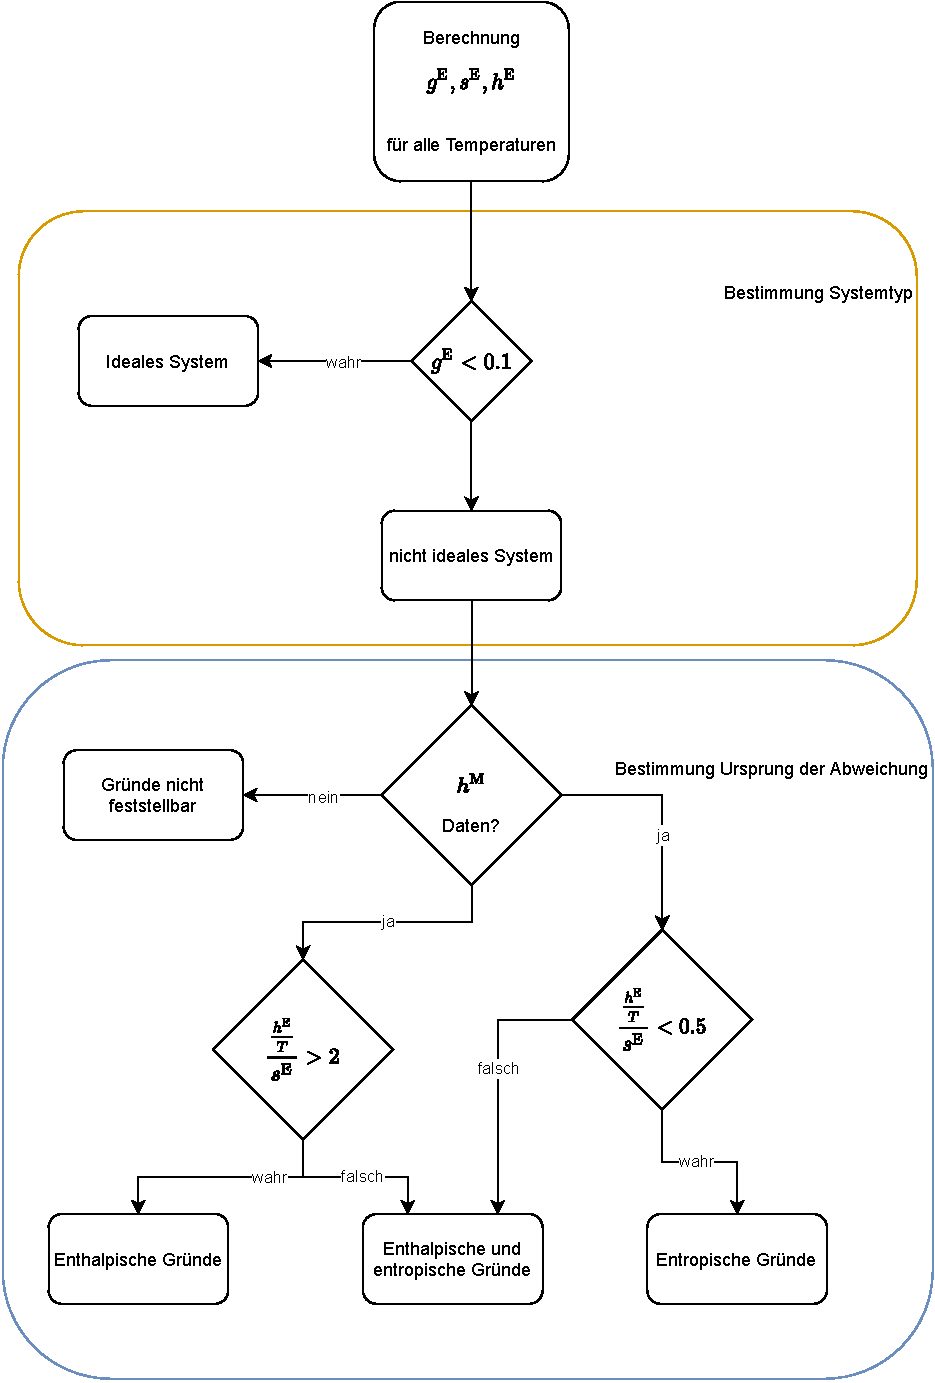
\includegraphics[scale=0.65]{Idealverhalten.pdf}
	\caption{Routine zur Bestimmung des Verhalten eines Gemischs und falls notwendig Bestimmung des Ursprungs der Abweichung}
	\label{fig: klassifikation}
\end{figure}

\subsection{Bewertungskriterien und Bewertungsgrößen}

Um zwei thermodynamische Modelle miteinander zu vergleichen werden beide mit experimentellen Daten verglichen und die Abweichung als Bewertungskriterium benutzt. Der Vergleich mit experimentellen Daten wird im folgenden Abschnitt erläutert.

Zum Vergleich eines thermodynamischen Modells mit experimentellen Daten werden folgende Größen verwendet:
\begin{itemize}
	\item kritischer Druck
	\item kritische Zusammensetzung
	\item azeotroper Druck
	\item azeotrope Zusammensetzung
	\item Zusammensetzung Flüssigphase
	\item Zusammensetzung Dampfphase (oder zweite Flüssigphase)
	\item 3 Phasen Druck
	\item 3 Phasen Zusammensetzung
	\item Mischungsenthalpie
	\item Mischungswärmekapazität
\end{itemize}

Aufgrund der Gibbs'schen Phasenregel ergibt sich für alle Größen ein Freiheitsgrad > 0 sodass hierfür mindestens eine Größe festgelegt werden muss um die unbekannten berechnen zu können. Beispielhaft ist die Berechnung der Freiheitsgrade für den kritischen Punkt eines binären Gemischs in \autoref{eq: gibb p_krit} beschrieben.
Der kritische Punkt wird durch drei Größen eindeutig definiert:
\begin{itemize}
	\item Druck $p$
	\item Temperatur $T$
	\item Zusammensetzung $x_1$
\end{itemize}

Mit der Gibb'schen Phasenregel lässt sich der Freiheitsgrad für ein Gemisch aus zwei Fluiden wie folgt berechnen.

\begin{equation}
	\label{eq: gibb p_krit}
	f = K - P + 2 = 2 - 3 + 2 = 1
\end{equation}

Das Gemisch liegt am kritischen Punkt als Flüssigkeit, Dampf sowie im überkritischen Zustand vor.

In \autoref{tab: DoF} sind die festgelegten und berechneten Größen analog zu Tabelle 13 \cite{jaubert2020benchmark} aufgeführt.

\begin{table} [htb]
	\centering
	\caption{Festgelegte und Berechnete Größen für ein binäres System}
	\begin{tabular}{ cccc }
		\hline 
		Größe & Freiheitsgrad & festgelegte Größen & berechnete Größen\\
		\hline  \\ 
		[\dimexpr-\normalbaselineskip+2pt]
		kritischer Druck  & 1 &$T_{\mathrm{c}}$ & $p_{\mathrm{c}},x_{\mathrm{c}}$  \\
		kritische Zusammensetzung  & 1 &$T_{\mathrm{c}}$ & $p_{\mathrm{c}},x_{\mathrm{c}}$  \\
		azeotroper Druck  & 1 &$T$ & $p,x_1$  \\
		azeotrope Zusammensetzung  & 1 &$T$ & $p,x_1$  \\
		Zusammensetzung Flüssigphase & 2 & $T,p$ & $x_1,y_1$ \\
		Zusammensetzung Dampfphase & 2 & $T,p$ & $x_1,y_1$ \\
		3-Phasen-Druck & 1 & $T$ & $x_1^{\alpha},x_1^{\beta},y_1$ \\
		3-Phasen-Zusammensetzung & 1 & $T$ & $x_1^{\alpha},x_1^{\beta},y_1$ \\
		Mischungsenthalpie & - & $T,p,z_1$ & $h^{\mathrm{M}}$ \\
		Mischungswärmekapazität & - & $T,p,z_1$ & $c_{\mathrm{p}}^{\mathrm{M}}$ \\
		[\dimexpr-\normalbaselineskip+18pt]
		\hline
		\label{tab: DoF}
	\end{tabular}
\end{table}

Diese Größen werden für jedes Stoffgemisch falls möglich berechnet und mit den experimentellen Daten, falls sie erhoben worden sind, verglichen. Aus den Abweichung der Werte werden für jede BAC Gruppe Noten berechnet und schließlich die Gesamtnote aus den Teilnoten ermittelt.

\section{Notenberechnung}

In diesem Kapitel wird die Berechnung der Gesamtnote eines thermodynamischen Modells und auf die Berechnung einzelnen, dafür notwendigen, Teilnoten eingegangen.

\subsection{Berechnung der Gesamtnote}
Die maximale Punktzahl die ein Modell ereichen kann ist auf 20 festgelegt. Die Gesamtnote wird aus vier einzelnen Teilnoten berechnet. Diese vier Teilnoten werden für jede Art der auftretenden Interaktion wie in \autoref{sec: klassifikation} beschrieben.

\begin{equation}
	\mathrm{mark}_{\mathrm{final}} = \dfrac{1}{4} \cdot \left( 
		\mathrm{mark}_{\mathrm{NA}} + \mathrm{mark}_{\mathrm{SA}} + \mathrm{mark}_{\mathrm{CA}} + \mathrm{mark}_{\mathrm{CA + SA}} 
	 \right)
\end{equation}

Die einzelnen Teilnoten wie z.B. $mark_{\mathrm{NA}}$ entsprechen den Noten der in \autoref{tab: bin-bac} aufgeführten Klassen. Die Noten der einzelnen Klassen berechnen sich aus den Mittelwerten der Noten der BAC Gruppen. Die Note für nicht-assoziative Gemsiche lässt sich beispielsweise wie folgt berechnen:

\begin{equation}
	\mathrm{mark}_{\mathrm{NA}} = \dfrac{1}{4} \cdot \left(
		\mathrm{mark}_{\mathrm{BAC_1}} + \mathrm{mark}_{\mathrm{BAC_2}} + \mathrm{mark}_{\mathrm{BAC_3}} + \mathrm{mark}_{\mathrm{BAC_4}}
	\right)
\end{equation}

Die Berechnung der Noten der drei weiteren Klassen erfolgt analog mit der in \autoref{tab: bin-bac} dargestellten Einteilung.

\subsection{Berechnung des Gemittelten durchschnittlichen Fehlers}
In diesem Abschnitt wird die Berechnung des gemittelten durchschnittlichen Fehlers gezeigt, welcher auch als \textbf{M}ean \textbf{A}verage \textbf{P}ercantage \textbf{E}rror oder kurz MAPE bezeichnet wird.

Die Berechnung dieser Größe wird am Beispiel der Größe XYZ für das Gemisch ABC gezeigt.

\subsection{Berechnung der Noten für die Bewertungsgrößen}
Die einzelnen Teilnoten werden aus den Noten der jeweiligen Bewertungsgrößen bestimmt.
\\

Die Note für den kritischen Druck errechnet sich mit folgendem Zusammenhang.
\begin{equation}
	\mathrm{Mark}_{p_{\mathrm{c}}} = 20 - 0,75 \cdot \mathrm{MAPE}_{p_\mathrm{c}}(\%)
\end{equation}

$ p_\mathrm{c} $ ist der Druck am kritischen Punkt.
\\
Die Note für die kritische Zusammensetzung wird nach \autoref{eq: mark_x_c} berechnet.
\begin{equation}
\label{eq: mark_x_c}
\mathrm{Mark}_{\mathrm{x_\mathrm{c},y_\mathrm{c}}} = 20 - 0,5 \cdot \left[
	\dfrac{\mathrm{MAPE_{x_{1,\mathrm{c}},y_{1,\mathrm{c}}}}(\%) + \mathrm{MAPE_{x_{2,\mathrm{c}},y_{2,\mathrm{c}}}}(\%)}{2}
\right]
\end{equation}

Die Größen $ x_{1,\mathrm{c}} $ und $ y_{1,\mathrm{c}} $ beschreiben die Molenbrüche für die erste Komponente in der Flüssig- und der Gasphase am kritischen Punkt. Die Größen mit dem Index 2 beziehen sich auf die anaolg auf die zweite Komponente.
\\

Für den azeotropen Druck kann die Note wie folgt berechnet werden.
\begin{equation}
	\mathrm{Mark}_{p_{\mathrm{az}}} = 20 - 0,5 \cdot \mathrm{MAPE}_{p_\mathrm{az}}(\%)
\end{equation}

$ p_\mathrm{az} $ bezeichnet den Druck am azeotropen Punkt.
\\

Für die azeotrope Zusammensetzung gilt folgender Zusammenhang.
\begin{equation}
\mathrm{Mark}_{\mathrm{x_\mathrm{az},y_\mathrm{az}}} = 20 - 0,5 \cdot \left[
	\dfrac{\mathrm{MAPE_{x_{1,\mathrm{az}},y_{1,\mathrm{az}}}(\%)} + \mathrm{MAPE_{x_{2,\mathrm{az}},y_{2,\mathrm{az}}}}(\%)}{2}
\right]
\end{equation}

Die Größen $ x_{1,\mathrm{az}} $ und $ y_{1,\mathrm{az}} $ beschreiben die Molenbrüche der ersten Komponente in der Flüssig- und der Gasphase am azeotropen Punkt.
\\

Die Noten für die Phasengleichgewichtsgrößen werden mit folgender Gleichung bestimmt.
\begin{equation}
	\mathrm{Mark}_{\mathrm{x,y}} = 20 - 0,5 \cdot \left[
		\dfrac{\mathrm{MAPE_{x_1,y_1}(\%)} + \mathrm{MAPE_{x_2,y_2}}(\%)}{2}
	\right]
\end{equation}

$x_1$ ist die Zusammensetzung der ersten und $x_2$ die des zweiten Stoffs in der Flüssigphase. Die Größen $ y $ beschreiben die Zusammensetzung in der Gasphase.

Die Note für die Mischungsenthalpie $ h^{\mathrm{M}} $ wird aus den Abweichungen der einzelnen Datenpunkte nach \autoref{} errechnet.
\begin{equation}
\mathrm{Mark}_{h^{\mathrm{M}}} = 20 - 0,25 \cdot \dfrac{1}{n_{h^{\mathrm{M}}}} \sum_{i=1}^{n_{h^{\mathrm{M}}}}
	\dfrac{1}{2} \cdot \left[
		100 \cdot \biggl|
			\dfrac{h_i^{\mathrm{M,EXP}}-h_i^{\mathrm{M,MODEL}}}{h_i^{\mathrm{M,EXP}}} 
			\biggl| 
			+ 100 \cdot \biggl| \dfrac{h_i^{\mathrm{M,EXP}}-h_i^{\mathrm{M,MODEL}}}{h_i^{\mathrm{M,MODEL}}}
		\biggl|
	\right]
\end{equation}

Um Noten die kleiner als null werden auszuschließen wird für Abweichungen aus dem Term
\begin{equation}
	\label{eq: h_m MAPEs}
	\dfrac{1}{2} \cdot \left[
	100 \cdot \biggl|
	\dfrac{h_i^{\mathrm{M,EXP}}-h_i^{\mathrm{M,MODEL}}}{h_i^{\mathrm{M,EXP}}} 
	\biggl| 
	+ 100 \cdot \biggl| \dfrac{h_i^{\mathrm{M,EXP}}-h_i^{\mathrm{M,MODEL}}}{h_i^{\mathrm{M,MODEL}}}
	\biggl| \right] > 80
\end{equation}
die Abweichung auf 80 \% festgesetzt. Dies führt zu einer Note von 0/20 für Punkte, welche die Bedingung erfüllen. Eine weitere zu berücksichtigende Schwierigkeit ist, dass große Abweichungen des Modelwerts vom experimentell ermittelten Wert abhängig davon ob sie nach oben oder unten abweichen, zu unterschiedlichen prozentualen Abweichungen führen.
Als Beispiel sind zwei verschieden Fälle zu betrachten
\begin{enumerate}
	\item $ h_i^{\mathrm{M,EXP}} = 10 \mathrm{\frac{J}{mol}} $ und $ h_i^{\mathrm{M,MODEL}} = 1000 \mathrm{\frac{J}{mol}} $
	\item $ h_i^{\mathrm{M,EXP}} = 1000 \mathrm{\frac{J}{mol}} $ und $ h_i^{\mathrm{M,MODEL}} = 10 \mathrm{\frac{J}{mol}} $
\end{enumerate}
Die Ergebnisse der Berechnung des MPAE sind \autoref{MPAE Glg} folgend wie folgt:
\begin{eqnarray}
MPAE_1 = 99 \rightarrow 9900 \% \\
MPAE_2 = 0.99 \rightarrow 99 \%
\end{eqnarray}

Um dieses Problem zu beheben wird der Mittelwert aus zwei MAPE wie in \autoref{eq: h_m MAPEs} gezeigt berechnet.

Die Note für die spezifische isobare Wärmekapazität wird mit dem gleichen Vorgehen, wie bei der Mischungswärmekapazität berechnet.
\begin{equation}
\mathrm{Mark}_{c_p{\mathrm{M}}} = 20 - 0,10 \cdot \dfrac{1}{n_{c_p{\mathrm{M}}}} \sum_{i=1}^{n_{c_p{\mathrm{M}}}}
\dfrac{1}{2} \cdot \left[
100 \cdot \biggl|
\dfrac{c_{p,i}^{\mathrm{M,EXP}}-c_{p,i}^{\mathrm{M,MODEL}}}{c_{p,i}^{\mathrm{M,EXP}}} 
\biggl| 
+ 100 \cdot \biggl| \dfrac{c_{p,i}^{\mathrm{M,EXP}}-c_{p,i}^{\mathrm{M,MODEL}}}{c_{p,i}^{\mathrm{M,MODEL}}}
\biggl|
\right]
\end{equation}
Um auch hier keine Noten kleiner als null zuzulassen wird für alle Punkte, welche die Bedingung 
\begin{equation}
\dfrac{1}{2} \cdot \left[
100 \cdot \biggl|
\dfrac{c_{p,i}^{\mathrm{M,EXP}}-c_{p,i}^{\mathrm{M,MODEL}}}{c_{p,i}^{\mathrm{M,EXP}}} 
\biggl| 
+ 100 \cdot \biggl| \dfrac{c_{p,i}^{\mathrm{M,EXP}}-c_{p,i}^{\mathrm{M,MODEL}}}{c_{p,i}^{\mathrm{M,MODEL}}}
\biggl| \right]> 200
\end{equation}
erfüllen die Abweichung auf 200 \% festgesetzt.

\begin{table} [htb]
	\centering
	\caption{Festgelegte und Berechnete Größen für ein binäres System}
	\begin{tabular}{ cc }
		\hline 
		Größe & Gewicht \\
		\hline  \\ 
		[\dimexpr-\normalbaselineskip+2pt]
		kritischer Druck  & 0,75   \\
		kritische Zusammensetzung  & 0,5   \\
		azeotroper Druck  & 0,5  \\
		azeotrope Zusammensetzung  & 0,5  \\
		Zusammensetzung Flüssigphase & 0,5 \\
		Zusammensetzung Dampfphase & 0,5 \\
		3-Phasen-Druck 0,5 &  \\
		3-Phasen-Zusammensetzung & 0,5  \\
		Mischungsenthalpie & 0,25 \\
		Mischungswärmekapazität & 0,10 \\
		[\dimexpr-\normalbaselineskip+18pt]
		\hline
		\label{tab: Notengewichte}
	\end{tabular}
\end{table}

Aus \autoref{tab: Notengewichte} geht hervor, dass der kritische Druck den größten Einfluss der einzelnen Teilnoten hat, da dieser die Topologie des Gemischs bestimmt. Das geringeste Gewicht habe die Mischungswärmekapazität und die Mischungsenthalpie, da diese in der Anwendung auch bei prozentualen Abweichungen von 20 bis 50 \% nur einen geringen Einfluss auf das Berechnungsergebniss haben.


\end{document}
